\section{General Description}
The NDLS module stands for the nuclear data library system, which stores all ENDF-6 formatted data in a database. The benefit of this approach instead of traditional text file of ENDF is that it supports multi-processes access or even multi-operating systems access to database. So many applications can share the same database. The database supports regular SQL query interfaces, so it may be familiar to the existing client program. 

\section{Database ER Diagram and Schema}
The NDLS uses a database management system (DBMS) to store the ENDF data. The basic unit in a DBMS is a table, which contains rows of data with a homogenous column structure, i.e. a spreadsheet in Excel. To make the ENDF data fits in a database, we furthers break the data into more fundamental units. These units are represented in great details in an Entity-Relationship (ER) diagram and the schema of each table, and give the receipt how to store the ENDF information in terms of entries in the tables in DBMS. For one looks for how to use the programming API, one can skip this section.

\subsection{ER Diagram}
The design of a database can be described by a graph called Entity-Relationship (ER) diagram. This section describes the design. The database contains  7 entities: Material, Description, Type, Header, Function, List, and Interpolation entities. Next we describe their meaning and the relationship between them in details.

The top level abstraction of objects in the database is a material, which is associated with a material number (MAT). According to ENDF-6 format, an evaluated material is uniquely defined by the following numbers:

\begin{itemize}
\item MAT: a  unique identifier for a nuclide whose cross sections are evaluated in the database
\item NLIB: an integer indicating from where the file evaluated, such as ENDF/B, CENDL, JENDL,
\item NVER: an integer indicating the major version of the evaluation,
\item LREL: an integer indicating the minor release version of the evaluation,
\item NSUB: an integer indicating the type of collections of the evaluation,
\item NMOD: an integer indicating the modification flag,
\item LDRV: an integer indicating the derivation flag for a given material,
\item TEMP: a real number indicating the temperature of the material of evaluation.
\end{itemize}

Each material has a description associating with it. The description contains the following fields:
\begin{itemize}
\item ZSYMAM: the chemical symbol of the nuclide,
\item ALAB:  the originating laboratory,
\item EDATE: the date of evaluation,
\item AUTH: the authors names,
\item REF: primary reference information,
\item DDATE: original distribution date,
\item RDATE: the data and number of last version to this evaluation,
\item ENDATE: the master file entry date,
\item HSUB: first few rows of evaluation metadata,
\item Summary: some conclusive sentences about the evaluation,
\item Description: additional comments given in the evaluation file.
\end{itemize}
Since each description is uniquely associated with a material, and a material evaluation has a description, there is a one-to-one the relationship between the material entity and the description entity. 

Each material evaluation contains files the are identified by the file number (MF) and the reaction number (MT). We call the combination of the (MF, MT) pair as the properties of a type entity. There are multiple type entities associating with a material. 

\begin{figure}[h]
\begin{center}
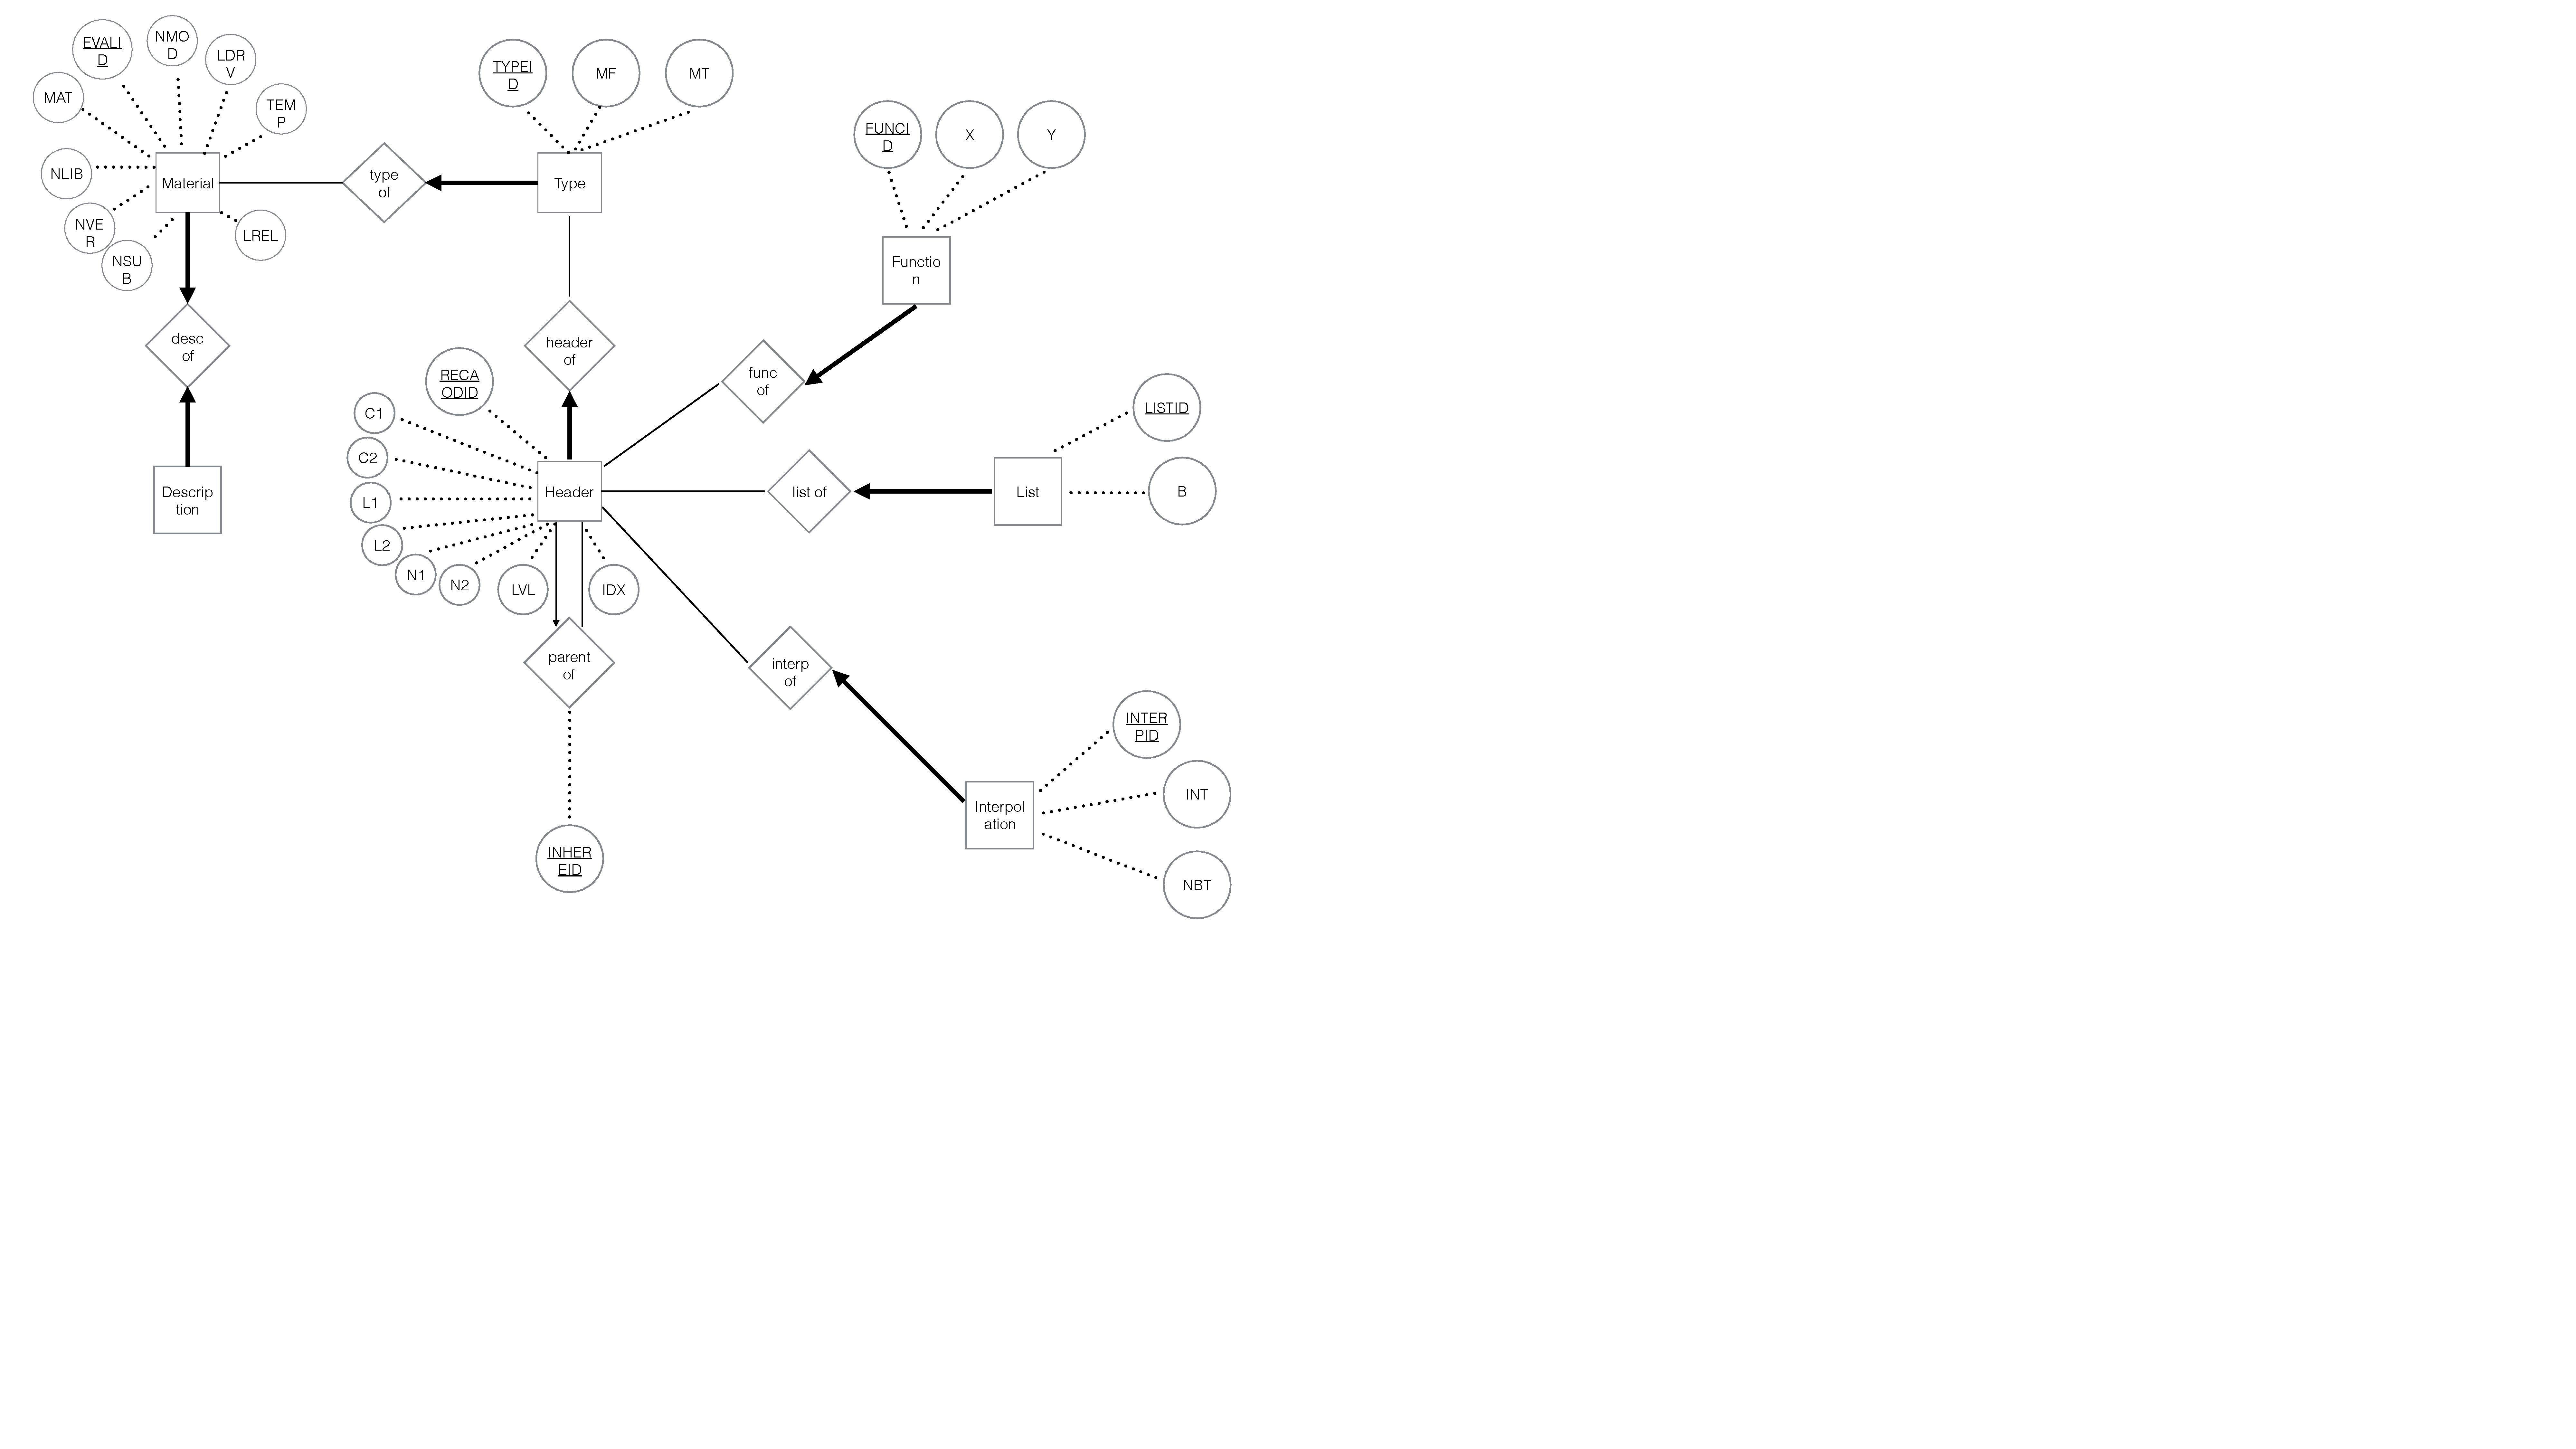
\includegraphics[scale=0.2]{./pics/endf-er-diagram.pdf}
\end{center}
\caption{ \label{fig:endf-6-record-tab2}
The ER diagram of the database}
\end{figure}

A header entity corresponds to a CONT record in the ENDF file, which contains six properties: C1, C2, L1, L2, N1, N2. In the ENDF text file, each CONT record is followed by any information for a list,  a one-dimensional function or a two dimensional function. The abstractions of function, list or interpolation entities, discussed later, are designated to describe a ENDF list, one-dimensional function, or a two dimensional function. Then in the ENDF file, a header entity is followed by a function, a list, an interpolation entity, or another header entity. An illustration of the file structure is shown in Figure \ref{fig:endf-header-inheritance}

\begin{figure}[h]
\begin{center}
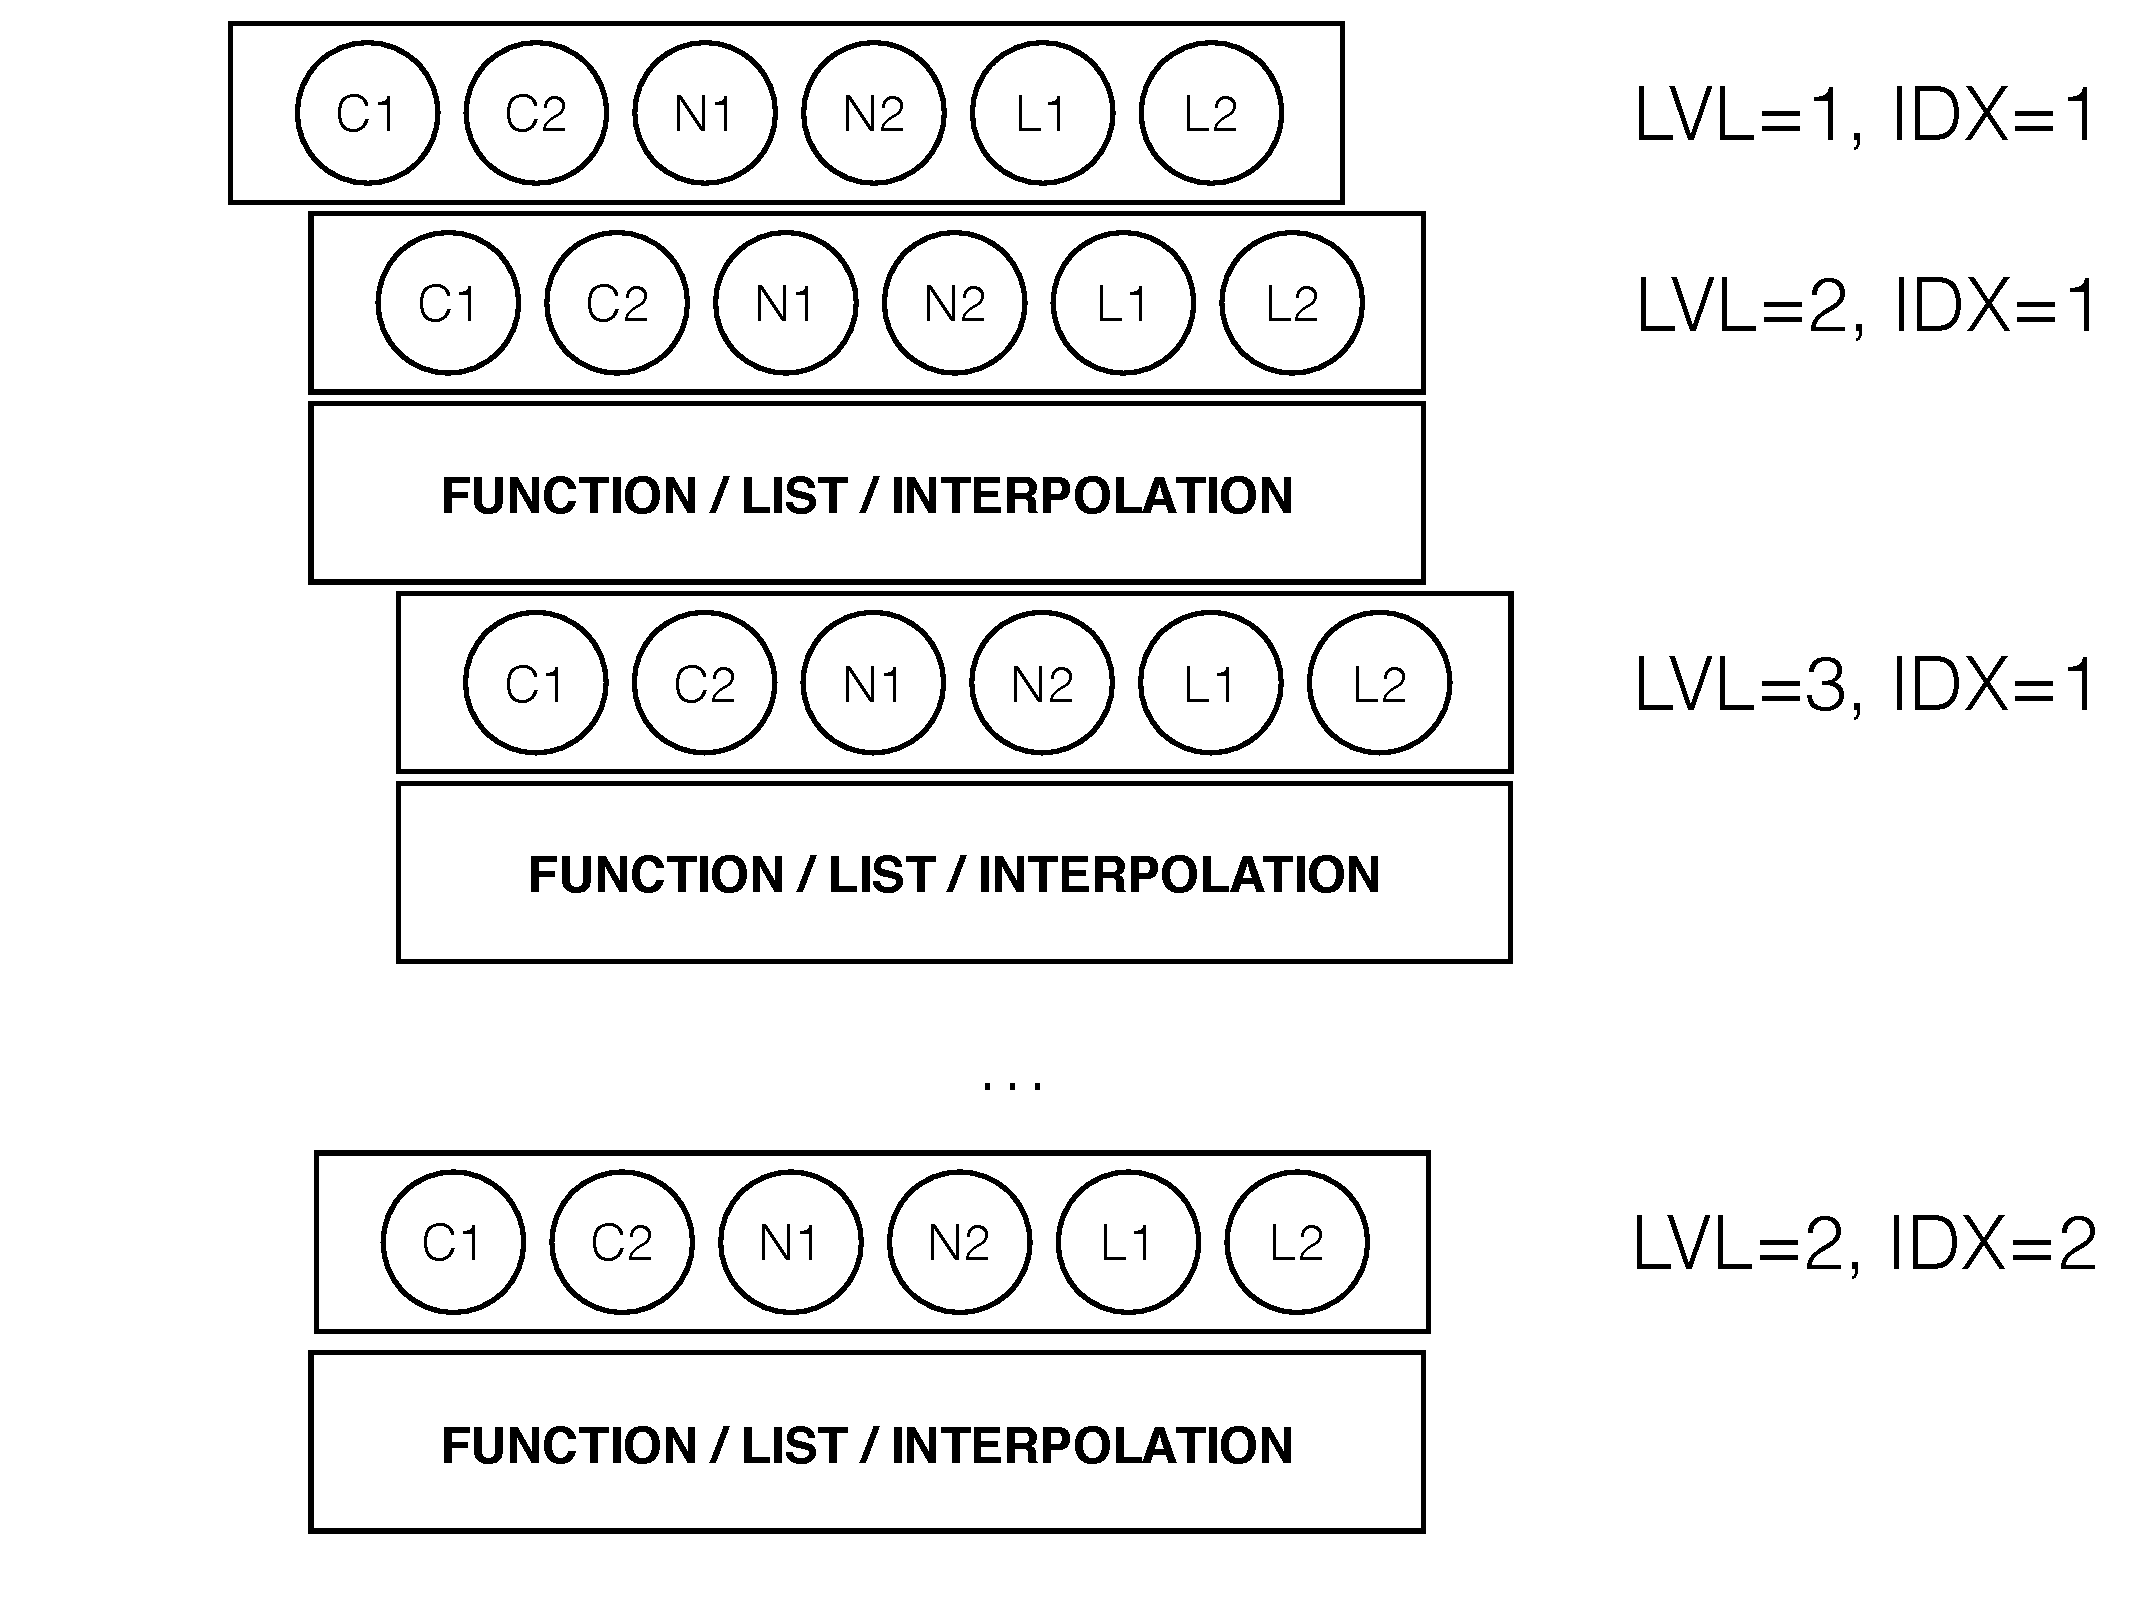
\includegraphics[scale=0.3]{./pics/endf-header-inheritance.pdf}
\end{center}
\caption{ \label{fig:endf-header-inheritance}
The header entities and the entities followed}
\end{figure}

Since a header entity could follow another header entity, there is an inherence relationship between the header entities. So we assign another two properties: the level (LVL) and the index (IDX) to indicate the parent-children relationship between headers and the brother and sister relationship between the header entities within a level. 

A function entity contains two properties x and y, which describe a one-dimensional function. A list entity contains a property B, which describes an array of data. An interpolation entity contains two properties: NBT and INT, which is used to describe the ENDF interpolation law. 

In the following sections, the database schema are given in more details.

\subsection{Material Table}
The material table contains important evaluation conditions for all evaluated data. According to the NJOY document, each evaluated data has a unique combination of MAT, NLIB, NVER, LREL, NSUB, NMOD, LDRV, and TEMP. We chose a self increasing integer EVALID as the primary key, which is generated at the time of inserting data into the database. The schema is shown in Program \ref{program:material_table_schema}.
\begin{program}[!htb]
\centering
\begin{verbatim} 
CREATE TABLE `Material_Table` (
	`EVALID`	INTEGER NOT NULL,
	`MAT`	INTEGER NOT NULL,
	`NLIB`	INTEGER NOT NULL,
	`NVER`	INTEGER NOT NULL,
	`LREL`	INTEGER NOT NULL,
	`NSUB`	INTEGER NOT NULL,
	`NMOD`	INTEGER NOT NULL,
	`LDRV`	INTEGER NOT NULL,
	`TEMP`	REAL NOT NULL,
	PRIMARY KEY(EVALID)
);
\end{verbatim}
\caption{ \label{program:material_table_schema}
SQL schema for material table}
\end{program}

\subsection{Description Table}
The description table includes additional evaluation information of the evaluated data. The EVALID from the material table is the primary key. The schema is shown in Program \ref{program:description_table_schema}.
\begin{program}[!htb]
\centering
\begin{verbatim} 
CREATE TABLE `Description_Table` (
	`EVALID`	INTEGER NOT NULL UNIQUE,
	`ZSYMAM`	TEXT,
	`ALAB`	TEXT,
	`EDATE`	TEXT,
	`AUTH`	TEXT,
	`REF`	TEXT,
	`DDATE`	TEXT,
	`RDATE`	TEXT,
	`ENDATE`	TEXT,
	`HSUB`	TEXT,
	`Summary`	TEXT,
	`Description`	TEXT,
	PRIMARY KEY(EVALID),
	FOREIGN KEY(`EVALID`) REFERENCES `Material_Table`(`EVALID`)
);
\end{verbatim}
\caption{ \label{program:description_table_schema}
SQL schema for description table}
\end{program}

\subsection{Type Table}
The type tables includes all file section paris. A self increasing integer TYPEID is automatically generated at the time of inserting data into the database and serve as the primary key. The schema is shown in Program \ref{program:type_table_schema}.

\begin{program}[!htb]
\centering
\begin{verbatim} 
CREATE TABLE `Type_Table` (
	`TYPEID`	INTEGER NOT NULL,
	`EVALID`	INTEGER NOT NULL,
	`MF`	INTEGER NOT NULL,
	`MT`	INTEGER NOT NULL,
	PRIMARY KEY(TYPEID),
	FOREIGN KEY(`EVALID`) REFERENCES `Material_Table`(`EVALID`)
);
\end{verbatim}
\caption{ \label{program:type_table_schema}
SQL schema for type table}
\end{program}

\subsection{Header Table}
The header table gives the header information for each record. A self increasing integer RECORDID is automatically generated at the time of inserting data into the database and serve as the primary key. The schema is shown in Program \ref{program:header_table_schema}.
\begin{program}[!htb]
\centering
\begin{verbatim} 
CREATE TABLE `Header_Table` (
	`RECORDID`	INTEGER NOT NULL,
	`TYPEID`	INTEGER NOT NULL,
	`C1`	REAL NOT NULL,
	`C2`	REAL NOT NULL,
	`L1`	REAL NOT NULL,
	`L2`	REAL NOT NULL,
	`N1`	REAL NOT NULL,
	`N2`	REAL NOT NULL,
	`LVL`	INTEGER NOT NULL,
	`IDX`	INTEGER NOT NULL,
	PRIMARY KEY(RECORDID),
	FOREIGN KEY(`TYPEID`) REFERENCES `Type_Table`(`TYPEID`)
);
\end{verbatim}
\caption{ \label{program:header_table_schema}
SQL schema for header table}
\end{program}

\subsection{Inheritance Table}
The inheritance table is designated to describe the inheritance relationship between the header tables, and the schema of which is shown in Program \ref{program:inherence_table_schema}.
\begin{program}[!htb]
\centering
\begin{verbatim} 
CREATE TABLE `Inheritance_Table` (
	`INHEREID`	INTEGER NOT NULL,
	`PARENTID`	INTEGER NOT NULL,
	`CHILDID`	INTEGER NOT NULL,
	PRIMARY KEY(INHEREID),
	FOREIGN KEY(`PARENTID`) REFERENCES `Header_Table`(`RECORDID`),
	FOREIGN KEY(`CHILDID`) REFERENCES `Header_Table`(`RECORDID`)
);
\end{verbatim}
\caption{ \label{program:inherence_table_schema}
SQL schema for inherence table}
\end{program}

\subsection{Function Table}
The function table records all one-dimensional functions x-y pairs. The RECORDID of a header table it associates with is the primary key. The schema of the function table is shown in Figure \ref{program:function_table_schema}.
\begin{program}[!htb]
\centering
\begin{verbatim} 
CREATE TABLE `Function_Table` (
	`FUNCID`	INTEGER NOT NULL,
	`RECORDID`	INTEGER NOT NULL UNIQUE,
	`X`	BLOB NOT NULL,
	`Y`	BLOB NOT NULL,
	PRIMARY KEY(FUNCID),
	FOREIGN KEY(`RECORDID`) REFERENCES `Header_Table`(`RECORDID`)
);
\end{verbatim}
\caption{ \label{program:function_table_schema}
SQL schema for function table}
\end{program}

\subsection{List Table}
The list table records all arrays of data in a list. The RECORDID of a header table it associates with is the primary key. The schema of the function table is shown in Figure \ref{program:list_table_schema}.
\begin{program}[!htb]
\centering
\begin{verbatim} 
CREATE TABLE `List_Table` (
	`LISTID`	INTEGER NOT NULL,
	`RECORDID`	INTEGER NOT NULL UNIQUE,
	`B`	BLOB NOT NULL,
	PRIMARY KEY(LISTID),
	FOREIGN KEY(`RECORDID`) REFERENCES `Header_Table`(`RECORDID`)
);
\end{verbatim}
\caption{ \label{program:list_table_schema}
SQL schema for list table}
\end{program}

\subsection{Interpolation Table}
The interpolation table records all ENDF interpolation rules. The RECORDID of a header table it associates with is the primary key. The schema of the function table is shown in Figure \ref{program:interpolation_table_schema}.
\begin{program}[!htb]
\centering
\begin{verbatim} 
CREATE TABLE `Interpolation_Table` (
	`INTERPID`	INTEGER NOT NULL,
	`RECORDID`	INTEGER NOT NULL UNIQUE,
	`INT`	BLOB NOT NULL,
	`NBT`	BLOB NOT NULL,
	PRIMARY KEY(INTERPID),
	FOREIGN KEY(`RECORDID`) REFERENCES `Header_Table`(`RECORDID`)
);
\end{verbatim}
\caption{ \label{program:interpolation_table_schema}
SQL schema for interpolation table}
\end{program}



%\section{Explicit Format Data-files}
%The information read from the database are too rudimentary and the meaning of the data are not disclosed explicitly. So we design the explicit format data-files to disclose the structural information of the nuclear data. The Google Protobuf format is used as a descriptive language for instantiating the nuclear data. In this section, we focus on the neutron data files.
%
%\subsection{Google Protobuf Message Format}
%The Google Protobuf protocol defines how to represent complex structured data. An example protocol message is shown in Program \ref{program:example_protocol}.
%
%\begin{program}[!htb]
%\centering
%\begin{verbatim} 
%message MessageName {
%modifier DataType variable = variable_index;
%}
%\end{verbatim}
%\caption{ \label{program:example_protocol}
%An example Google Protobuf protocol}
%\end{program}
%
%The 'messageName' variable is the name of the message or a structure. It is called a message because that the protocol file is used for sending data between computers in the Google cluster of servers. The 'modifier' field has three options, they are: required, repeated or optional, which modify the 'variable' after with type specified by 'DataType'. The data type can either be basic types such as a double precision floating number (double), a string (string), or  The 'variable\_index' is a unique integer for a variable in a message. This integer associates with the location of the variable when packed in an array of bytes.
%
%\subsection{Top Level Information for Neutron Data}
%The neutron data can be categorized into the resonance data (file 2), the reaction data (file 3), etc. The protocol is shown in Program \ref{program:top_level_neutron_data}.
%\begin{program}[!htb]
%\centering
%\begin{verbatim} 
%message NeutronData {
%	repeated Reaction reactions = 1;
%	repeated Resonance resonances = 2;
%}
%\end{verbatim}
%\caption{ \label{program:top_level_neutron_data}
%Google Protobuf protocol for top level information for neutron data}
%\end{program}
%
%\subsection{Fundamental ENDF data structures}
%The fundamental ENDF data structures include those for the ENDF tabulars and interpolation laws. The protocols are shown in Figure \ref{program:fundamental_endf_data_structure}.
%\begin{program}[!htb]
%\centering
%\begin{verbatim} 
%message TableInterpLaw {
%	required int64 INT = 1;
%	required int64 NBT = 2;
%}
%message TableDataPoint {
%	required double X = 1;
%	required double Y = 2;
%}
%message Table {
%	repeated TableInterpLaw interp_laws = 1;
%	repeated TableDataPoint data_points = 2;
%}
%\end{verbatim}
%\caption{ \label{program:fundamental_endf_data_structure}
%Google Protobuf protocol for fundamental ENDF data structures}
%\end{program}
%
%\subsection{Resonance Data}
%In this section, we disclose the design of resonance data. The resonance data are split into ranges of resonances. A resonance region can either be a resolved resonance region (RRR) or a unresolved resonance region (URR). 
%
%\subsubsection{Top Level Information for Resonance Data}
%The top level information for a resonance includes the atomic-mass number ZAI, the nuclide abundance ABN, the average fission width flag LFW, and an array of resonance ranges. The protocol is shown in Program \ref{program:top_level_neutron_data}.
%\begin{program}[!htb]
%\centering
%\begin{verbatim} 
%message Resonance {
%	required int64 ZAI = 1;
%	required double ABN = 2;
%	required int64 LFW = 3;
%	repeated ResonanceRange ranges = 4;
%}
%\end{verbatim}
%\caption{ \label{program:top_level_resonance_data}
%Google Protobuf protocol for top level information for resonance data}
%\end{program}
%
%\subsubsection{Top Level Information for Resonance Range}
%For each resonance range, there are many parameters to describe. The top level information is listed below in Program \ref{program:top_level_resonance_range}. The EL variable is the lower bound of the energy range, and EH is the upper bound of the energy range. LRU is an integer flag indicates which this is a RRR with LRU equals to 1 or URR with LRU equals to 2. LRF is an integer flag indicating the format of evaluation of the resonance parameters: Single-Level Breit-Wigner representation (SLBW) with LRF equals to 1. Multi-Level Breit-Wigner representation (MLBW) with LRF equals to 2, Reich-Moore representation (RM) with LRF equals to 3, Adler-Adler representation (AA) wth LRF equals to 4, and R-Matrix Limited representation (RML) with LRF equals to 7. NRO is the flag for indicating the energy dependence of the scattering radius: energy independent with NRO equals to 0, or energy dependent with NRO equals to 1. NAPS is the flag controls the use of channel radius and the scattering radius (AP). 
%
%Next, it is discussed here the information only applicable to the resolved resonance region with LRU equals to 1. SPI is the spin of the target nucleus. AP is the scattering radius in units ${10^{-12}}$cm. APE is an ENDF table to store the energy dependent scattering radius. LAD (for RM) is a flag indicating whether parameters can be used to calculate angular distributions. NLSC (for RM) is the number of angular moments used for converging calculations. LI (for AA) is the flag for controlling the kind of AA parameters. NX (for AA) is the number of sets of background constants. AWRI is the ratio of the mass of the isotope to the mass of a neutron, i.e. the atomic weight ratio. 
%
%\begin{program}[!htb]
%\centering
%\begin{verbatim} 
%message ResonanceRange {
%	required double EL = 1;
%	required double EH = 2;
%	required int64 LRU = 3;
%	required int64 LRF = 4;
%	required int64 NRO = 5;
%	required int64 NAPS = 6;
%
%	required double SPI = 11;
%	required double AP = 12;
%	required Table APE = 13;
%	required int64 LAD = 14;
%	required int64 NLSC = 15;
%
%	required int64 LI = 21;
%	required int64 NX = 22;
%	required double AWRI = 23;
%
%	required int64 LSSF = 31;
%	repeated double URRBES = 32;
%
%	required int64 IFG = 41;
%	required int64 KRM = 42;
%	required int64 KRL = 43;
%	repeated RMLParticlePair RMLPairs = 44;
%	repeated RMLSpin RMLSpins = 45;
%
%	repeated double AATotal = 51;
%	repeated double AAFission = 52;
%	repeated double AACapture = 53;
%
%	repeated AngularMomentum moments = 61;
%}
%\end{verbatim}
%\caption{ \label{program:top_level_resonance_range}
%Google Protobuf protocol for top level information for resonance range}
%\end{program}
%
%The additional defined data structures protocols are listed in Program \ref{program:additional_resonance_parameters}, Program \ref{program:additional_resonance_parameters_cont}, Program \ref{program:additional_resonance_parameters_cont2}, and Program
%\ref{program:additional_resonance_parameters_cont3}.
%
%\begin{program}[!htb]
%\centering
%\begin{verbatim} 
%message BreitWigner {
%	required double ER = 1;
%	required double AJ = 2;
%	required double GT = 3;
%	required double GN = 4;
%	required double GG = 5;
%	required double GF = 6;
%}
%message ReichMoore {
%	required double ER = 1;
%	required double AJ = 2;
%	required double GN = 3;
%	required double GG = 4;
%	required double GFA = 5;
%	required double GFB = 6;
%}
%message AAResonance {
%	required double DET = 1;
%	required double DWT = 2;
%	required double GRT = 3;
%	required double GIT = 4;
%	required double DEF = 5;
%	required double DWF = 6;
%	required double GRF = 7;
%	required double GIF = 8;
%	required double DEC = 9;
%	required double DWC = 10;
%	required double GRC = 11;
%	required double GIC = 12;
%}
%message AdlerAdler {
%	required double AJ = 1;
%	repeated AAResonance resonaces = 2;
%}
%\end{verbatim}
%\caption{ \label{program:additional_resonance_parameters}
%Google Protobuf protocol for top level information for  addition resonance paramters}
%\end{program}
%
%\begin{program}[!htb]
%\centering
%\begin{verbatim} 
%message UrrA {
%	required double D = 1;
%	required double AJ = 2;
%	required double AMUN = 3;
%	required double GNO = 4;
%	required double GG = 5;
%}
%message UrrB {
%	required double L = 1;
%	required double MUF = 2;
%	required double D = 3;
%	required double AJ = 4;
%	required double AMUN = 5;
%	required double GNO = 6;
%	required double GG = 7;
%	repeated double GF = 8;
%}
%message UrrC {
%	required double AJ = 1;
%	required int64 INT = 2;
%	required double AMUX = 3;
%	required double AMUN = 4;
%	required double AMUG = 5;
%	required double AMUF = 6;
%	repeated double ES = 7;
%	repeated double D = 8;
%	repeated double GX = 9;
%	repeated double GNO = 10;
%	repeated double GG = 11;
%	repeated double GF = 12;
%}
%message AngularMomentum {
%	required double AWRI = 1;
%	required double QX = 2;
%	required double L = 3;
%	required int64 LRX = 4;
%	required double APL = 5;
%	repeated BreitWigner BWTables = 6;
%	repeated ReichMoore RMTables = 7;
%	repeated AdlerAdler AATables = 8;
%	repeated UrrA URRATables = 9;
%	repeated UrrB URRBTables = 10;
%	repeated UrrC URRCTables = 11;
%}
%\end{verbatim}
%\caption{ \label{program:additional_resonance_parameters_cont}
%Google Protobuf protocol for top level information for  addition resonance parameters (Continue)}
%\end{program}
%
%\begin{program}[!htb]
%\centering
%\begin{verbatim} 
%message RMLParticlePair {
%	required double MA = 1;
%	required double MB = 2;
%	required int64 ZA = 3;
%	required int64 ZB = 4;
%	required int64 IA = 5;
%	required int64 IB = 6;
%	required double Q = 7;
%	required int64 PNT = 8;
%	required int64 SHF = 9;
%	required int64 MT = 10;
%	required double PA = 11;
%	required double PB = 12;
%}
%message RMLChannel {
%	required double IPP = 1;
%	required double L = 2;
%	required double SCH = 3;
%	required double BND = 4;
%	required double APE = 5;
%	required double APT = 6;
%
%	required int64 LBK = 11;
%	required int64 LPS = 12;
%	required Table RBR = 13;
%	required Table RBI = 14;
%	required Table PSR = 15;
%	required Table PSI = 16;
%	required double R0 = 17;
%	required double S0 = 18;
%	required double R1 = 19;
%	required double S1 = 20;
%	required double R2 = 21;
%	required double EU = 22;
%	required double ED = 23;
%	required double GA = 24;
%}
%\end{verbatim}
%\caption{ \label{program:additional_resonance_parameters_cont2}
%Google Protobuf protocol for top level information for  addition resonance parameters (Continue)}
%\end{program}
%
%\begin{program}[!htb]
%\centering
%\begin{verbatim} 
%message RMLResonance {
%	required double ER = 1;
%	repeated double GAMS = 2;
%}
%message RMLSpin {
%	required double AJ = 1;
%	required double PJ = 2;
%	required int64 KBK = 3;
%	required int64 KPS = 4;
%	repeated RMLChannel RMLChannels = 5;
%	repeated RMLResonance RMLResonances = 6;
%}
%\end{verbatim}
%\caption{ \label{program:additional_resonance_parameters_cont3}
%Google Protobuf protocol for top level information for  addition resonance parameters (Continue)}
%\end{program}

%\subsection{Reaction Data}

\clearpage
\section{C++ Data Structure \& Application Interfaces}
The program is implemented native in C++ programming language, so in this section, we discuss the data structures first then the application interfaces.

\subsection{Data Structure}


\subsection{Application Interfaces (APIs)}
\begin{program}[!htb]
\centering
\begin{verbatim} 
class NDLS {
public:
    NDLS(const std::string& dbFilepath);
    ~NDLS();
    
    bool open(const std::string& dbFilepath);
    void close();
    bool insertENDFFile(const std::string& endfFilepath);
}
\end{verbatim}
\caption{ \label{program:ndls_cpp_api}
C++ public APIs for NDLS module}
\end{program}
